
The simplified DM models  defined in the last section  aim at capturing  accurately  the characteristics of MET production at high-energy colliders. They can be understood as a limit of a more general new-physics scenario, where all but the lightest dark-sector states are assumed to be sufficiently decoupled, so that only the interactions that are relevant at LHC energies are interactions between the mediator and DM as well as the SM quarks. 
Aside from this important caveat, a presentation of collider bounds in the simplified model framework requires no further assumptions, meaning  that LHC searches can be used to set model-independent bounds on the parameter space of a simplified model, and that the constraints arising from different channels --- e.g.~mono-jets and di-jets --- can be directly compared~(see for instance~\cite{Chala:2015ama}).  In this section, we spell out the model choices underlying the LHC limits and the relic density calculations.  
Issues arising in the DD and ID context are discussed in subsequent sections.


\subsection{Mass-mass plane}

\label{mass-massplane}

\begin{figure}[!t]
	\centering
	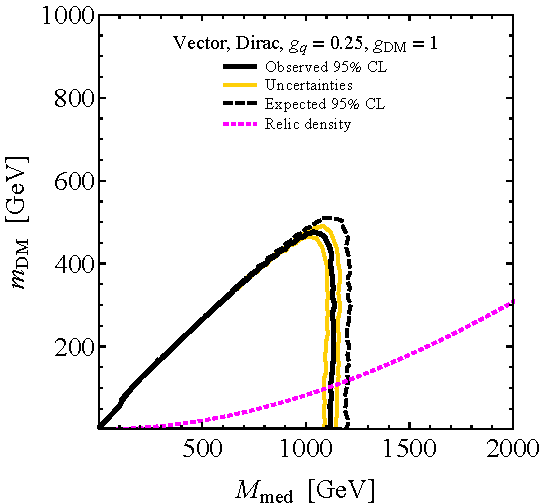
\includegraphics[width=0.6 \textwidth]{figure1.pdf}
	\caption{95\% CL exclusion contours in the mass-mass plane for a simplified model with a vector mediator, Dirac DM and couplings $\gq = 0.25$ and $\gDM = 1$. The black solid~(dashed) curve shows the median of the observed (expected) limit, while the yellow curves indicate an example of the uncertainties on the observed bound.  A minimal width is assumed and the excluded parameter space is to the bottom-left of all contours. The dotted magenta curve corresponds to the parameters where the correct DM relic abundance is obtained  from standard thermal freeze-out for the chosen couplings. DM is overproduced to the bottom-right of the curve. The shown  LHC results are intended for illustration only and are not based on real data. }   
	\label{fig:massmass}
\end{figure}

The advocated plots represent only two dimensional slices of the full four dimensional parameter space of the proposed simplified models. To allow for a qualitative understanding of the dependence of the results on the mediator couplings $\gq$ and $\gDM$,  we advocate an auxiliary figure that shows the limit on the ``signal strength'' $\mu$,~i.e.~the ratio of the experimental limit to the predicted signal cross section for fixed masses or fixed coupling scenarios.  We recommend however to clarify that a limit on $\mu$ must not be confused with a bound on a rescaling factor for the couplings and thus in general cannot be used to translate the exclusion limit in the mass-mass plane from one set of couplings to another. The reason is that changing $\gq$ and $\gDM$ typically modifies the total width of the mediator, which can change the kinematic distributions of the signal and thus the exclusion bounds in a non-trivial way. 
Furthermore, for scenarios where the mediator widths varies significantly as the function of the considered parameter (e.g. mass-mass plane), we suggest to add supporting material that illustrates the variation of the width in these parameters. 


The primary presentation recommended for LHC results in the simplified model language are plots of the experimental confidence level (CL) limits on the signal cross sections as a function of the two mass parameters $\mDM$ and $\mmed$  for a fixed set of couplings $\gq$ and~$\gDM$. An example of such a ``mass-mass" plot is given in Figure~\ref{fig:massmass}. It shows 95\%~CL exclusion limits (black and yellow curves) for the case of a vector mediator. The limits are derived from a hypothetical LHC mono-jet measurement. The particular choice of axes, with
 $\mmed$ on the $x$-axis and $\mDM$ on the  $y$-axis, follows the convention adopted when interpreting supersymmetry 
 searches at the LHC. The parameter space shown in the mass-mass plots can be divided into three regions: 

\begin{description}

\item[On-shell region:] The on-shell region, $\mmed > 2  \hspace{0.25mm}  \mDM$, is the region where  LHC searches for MET signatures provide the most stringent constraints. The production rate of the mediator decreases with increasing $\mmed$ and so does the signal strength in mono-jet searches. In this region the  experimental limits and the signal cross sections depend in a complex way on all parameters of the simplified model, and it is therefore in general not possible to translate the CL limit obtained for one fixed set of couplings $\gq$ and $\gDM$ to another by a simple rescaling procedure. 
	
 \item[Off-shell region:] In the off-shell region, $\mmed < 2 \hspace{0.25mm} \mDM$, pair-production of DM particles turns off and the constraints from MET searches rapidly lose power. The cross sections become proportional to the combination $\gq^2  \hspace{0.25mm} \gDM^2$ of couplings, so that in principle the LHC exclusions corresponding to different coupling choices can be derived by simple rescalings.  Deviations from this scaling are observed on the interface between on-shell and off-shell regions $\mmed \simeq 2 \hspace{0.25mm} \mDM$~\cite{Jacques:2015zha}. 
Note that for $\mmed < 2 \hspace{0.25mm} \mDM$ an on-shell mediator will always decay back to SM particles, meaning that the off-shell region can be probed by non-MET searches such as di-jets or di-tops. We also note that if the mediator is light and very weakly coupled to the SM quarks, constraints from DD and/or ID on these models may be typically stronger than those from the LHC.
 
  
\item[Heavy mediator limit:] The DM EFT limit is approached as the mediator mass $\mmed$ becomes large. In this limit the mono-jet cross sections scale with the fourth inverse power of the effective suppression scale $M_\ast =  \mmed/\sqrt{\gq \hspace{0.25mm} \gDM}$. For perturbative couplings (i.e.~$\sqrt{\gq  \hspace{0.25mm}  \gDM} \ll 4 \pi$), the EFT results apply to mediators with masses in the multi-TeV range. 

\end{description}

As in the template plot, any presentation of  the LHC limits has to clearly state the model assumptions made to obtain the exclusion contours. We thus advocate to explicitly specify on the figure the simplified model, including the mediator and DM type, and the choices of couplings. 
Besides the observed exclusion bound, the median of the expected limit and uncertainties (e.g.~those arising from scale variations or ambiguities related to the choice of parton distribution functions, as well as experimental uncertainties) are useful information that can be added to these plots. All these ingredients have been included in~Figure~\ref{fig:massmass}. 




The usefulness of the bound on $\mu$ is thus limited to cases where kinematic distributions are  the same for different realisations of the simplified model. Such a situation is realised for example in the on-shell region if all couplings are sufficiently small, so that the total decay  width of the mediator obeys $\Gamma_{\rm med} \lesssim 0.3 \hspace{0.25mm} \mmed$. Under these circumstances, one can use the narrow-width approximation~(NWA) to  show, for example, that in the case of a spin-1 mediator the mono-jet  cross section $\sigma ( p p \to \chi \bar \chi + j)$ factorises into mediator production $\sigma ( p p \to Z' + j)$ and the  invisible branching ratio ${\rm Br} (Z^\prime \rightarrow \chi\bar{\chi})$.  This factorisation implies that a bound on $\mu$ can be used to infer a limit  on the invisible branching ratio ${\rm Br} (Z^\prime \rightarrow \chi\bar{\chi})$ of the spin-1 mediator relative to the one in the benchmark model without regenerating  the underlying signal Monte Carlo (MC). Since the NWA can be an imperfect approximation even for weak couplings $\gq$ and $\gDM$ (see for instance~\cite{Jacques:2015zha}), we recommend that care is taken if relying on this argument.


If readers would like to reinterpret experimental limits for different coupling choices, it is their responsibility to ensure that kinematic distributions remain unchanged. To make this issue clear, we recommend that captions of plots showing limits on $\mu$  include a statement along the lines of ``Note that the bound on $\mu$ only applies to coupling combinations that yield the same kinematic distributions as the benchmark model.''.

\subsection{Choice of couplings for presentation of results in mass-mass plane}

\label{sub:couplingsandscaling}

At present, we recommend that mono-jet-like searches produce limits for a single choice of couplings. The ATLAS/CMS DM Forum report~\cite{Abercrombie:2015wmb} forms the basis of our recommendations for the simplified models given in Section~\ref{sec:models}. In particular, we advocate the following coupling values to produce the limits on signal strengths:
\begin{description}
\item[Vector mediator:] $\gDM=1$ and $\gq=0.25$.
\item[Axial-vector mediator:] $\gDM=1$ and $\gq=0.25$.
\item[Scalar mediator:] $\gq=1$ and $\gDM=1$.
\item[Pseudo-scalar mediator:] $\gq=1$ and $\gDM=1$.
\end{description}
The quark coupling $\gq$ should be universal in all cases and the width of the mediator should be set to the minimal width, meaning that it is assumed that the mediator has no couplings other than $\gq$ and $\gDM$.\footnote{Using the same value of $\gq$ for all quarks is theoretically well motivated for the vector, scalar and pseudo-scalar mediator. For the axial-vector mediator, it would also be interesting to consider $g_u = g_c = g_t = - g_d = -g_s = -g_b$, which arises naturally if the vector mediator corresponds to the massive gauge boson of a new broken $U(1)^\prime$ and the SM Yukawa couplings are required to be invariant under this additional gauge symmetry. The relative sign between the coupling to up-type 
and down-type quarks is important if interference plays a role and affects the comparison between LHC and  DD results.} The choices above provide for a consistent comparison across collider results within a given simplified model. They ensure that the mediator has $\Gamma_{\rm med}/M_{\rm med} \lesssim 10\%$ and that the theory is far from the strong coupling regime. The choice of $\gq=0.25$ for spin-1 mediators is furthermore motivated by the requirement to avoid di-jet constraints from the LHC and earlier hadron colliders (see e.g.~\cite{Chala:2015ama}). When readers are interested in extrapolating the provided results to other coupling values, it is their responsibility to understand how changing $\gq$ and $\gDM$ will affect the kinematics of the signal and therefore the experimental CL limits. To facilitate such an extrapolation, ATLAS and CMS could provide additional information (e.g.~tables of acceptances, efficiencies, number of events generated, total experimental uncertainty, number of events passing analysis cuts for benchmark signals)
corresponding to the recommended coupling choices as supplementary material, as detailed in Appendix B of~\cite{Abercrombie:2015wmb}. 
As discussed in~\cite{Abercrombie:2015wmb}, the kinematics of vector and axial-vector models is very similar in the case of jet radiation. The same consideration applies for the scalar and pseudo-scalar models in the mono-jet channel, while differences are seen for heavy flavour final states. 

\subsection{Overlaying additional information on LHC results}
\label{sec:overlayingadditionalinformation}

Fixing both $\gq$ and $\gDM$ has the advantage that, in a given model, one can compare the LHC results to relic density calculations or the limits obtained by  DD and ID experiments. Nevertheless, such comparisons typically 
require additional assumptions and should be done carefully. We discuss a few possibilities below. In all cases, we recommend to keep the plots simple, and to specify the assumptions clearly or to produce several variations to indicate the impact that different assumptions have on the final results. 

\subsubsection{Relic density}
\label{sub:relicdensity}

Relic density calculations can be overlaid on the mass-mass plot to indicate where the particles and interactions of a specific simplified model are by themselves sufficient for explaining the observed DM abundance.  For the simplified models recommended by the ATLAS/CMS DM Forum, this curve corresponds to the parameters for which the observed relic abundance is compatible with a single species of DM Dirac fermion and a single mediator that couples to all SM quarks with equal strength. One should not conclude that a simplified model is ruled out for values of model parameters that are inconsistent with the relic density overlay. Rather, one should conclude that additional physics beyond the simplified model was relevant for determining the DM abundance in the early Universe. 

When calculating the relic density, we recommend to include all tree-level processes relevant for the DM annihilation.  In particular, when $\mmed < \mDM$,
annihilation into on-shell mediators are typically active, and are particularly important when $\gDM \gg \gSM$ (e.g.~\cite{Abdullah:2014lla}), for
which cross sections are typically insensitive to $\gSM$, unlike LHC processes.

Numerical tools, such as {\tt micrOMEGAs}~\cite{Belanger:2014vza} and {\tt MadDM}~\cite{Backovic:2015cra}, can be used to calculate the regions of relic overproduction or underproduction for the simplified models recommended by the ATLAS/CMS DM Forum. We provide the results of {\tt MadDM}~calculations for the models described in Section~\ref{sec:models} at~\cite{relic_results}.  These results were obtained using the coupling values specified in Section~\ref{sub:couplingsandscaling}.  The reader should be aware that the axial-vector calculation does not include an explicit constraint from perturbative unitarity (described below).  The provided curves correspond to $\Omega_{\chi}h^{2}=0.12$ (the relic DM density observed by WMAP~\cite{Hinshaw:2012aka} and Planck~\cite{Ade:2015xua}) for the models considered.  Larger mediator masses as well as smaller DM masses (below the curves) correspond to larger values of $\Omega_{\chi}h^{2}$ (and conversely for smaller mediator masses and larger DM masses).


\subsubsection{Perturbativity limits, anomalies and issues with gauge invariance}
\label{sub:perturbativitylimit}


The couplings recommended by the ATLAS/CMS DM Forum have been fixed to values which are perturbative, with the mediator width always sufficiently smaller than the mediator mass. However, it was shown in~\cite{Chala:2015ama, Kahlhoefer:2015bea} that perturbative unitarity is violated in the axial-vector model due to the DM Yukawa coupling becoming non-perturbative, even for perturbative values of $g_q$ and $g_\text{DM}$, if $\mDM$ is significantly larger than $\mmed$.  It was argued that this consideration implies $m_\text{DM}^2 \gDM^2 / (\pi \mmed^2) < 1/2$,
which yields $m_\text{DM} < \sqrt{\pi / 2} \hspace{0.25mm} \mmed$ for the recommended value $\gDM = 1$. It is therefore proposed to indicate the line corresponding to $\mDM = \sqrt{\pi / 2} \hspace{0.25mm} \mmed$ in the mass-mass plot for the axial-vector case in a similar style as for the relic density constraint (i.e.~just a line, no shading). 



Another potential problem of the  vector and axial-vector model  is that they are not anomaly free if the $Z^\prime$ boson  couples only to quarks but not to leptons. This  implies that the full theory that ultraviolet completes (\ref{eq:AV1}) and  (\ref{eq:AV2}) must include new fermions to cancel the anomalies. While these fermions can be vector-like with respect to the SM, they will need to be chiral with respect to the new gauge group that gives rise to the~$Z^\prime$. In consequence, the  additional fermions  must have masses of the order of the symmetry-breaking scale, which  is at most a factor of a few above $M_{\rm med}$ \cite{Kahlhoefer:2015bea}.  While the existence of additional fermions will lead to new signatures, the precise impact on LHC phenomenology depends on the specific way the anomalies are cancelled. The resulting model dependence is difficult to quantify and we thus propose to ignore the issue of anomalies until it has been studied in detail by theorists. 

The interactions between the spin-0 mediator and the quarks present in the simplified scalar model are not $SU(2)_L$ invariant. As a result, these interactions will violate perturbative unitarity at high energies in tree-level process like $pp \to W + \phi \, (\phi \to \chi \bar \chi)$. The corresponding amplitudes are however proportional to the squares of the light-quark Yukawa couplings, so that in practice unitarity-violating effects are expected to have a negligible impact on the outcome of MET searches at the LHC. Still in $SU(2)_L$ invariant theories that provide specific realisation of the $s$-channel scalar mediator interactions~(\ref{eq:Scalar}),  like for instance the fermion singlet DM model (see~e.g.~\cite{Abdallah:2015ter}), the resulting LHC phenomenology can be modified by the new fields that are needed to make the full theory gauge invariant. These modifications are again model dependent and lacking detailed theoretical studies, their effect on the  LHC bounds cannot yet be quantified. 


\subsubsection{Additional plots}
\label{additionalplot}

Above, we recommend that LHC searches present the mass-mass plot, fixing both $\gq$ and $\gDM$, as the primary result. If desired, additional information on the coupling dependence of the results can be conveyed by producing a related set of limits where one of the mass parameters and one of the couplings has been fixed, and the other mass parameter and coupling are varied. As discussed in the previous section, a correct treatment of varying couplings is one which correctly accounts for the varying acceptance of the search.


\subsubsection{Non-collider DM searches}
\label{sub:non-colliderdmsearches}


Interpreting non-collider results  in the simplified model framework involves additional assumptions, and generally requires detailed knowledge of how the non-collider results were produced.
For example, as discussed above, the relic density predicted by the simplified model varies from point to point on the mass-mass plot, whereas non-collider results are typically presented under the assumption that the density of the DM particle under consideration saturates the cosmological density (i.e.\ that there is just one species of DM). These assumptions may be consistent if there is additional physics (not captured by the simplified model) that affects the relic density calculation but is irrelevant to the LHC signals~(see e.g.~\cite{Gelmini:2010zh}). However, it is also a possibility that the DM particle probed by non-collider experiments constitutes only a certain component of the DM density, so their results would have to be rescaled accordingly (see~for instance~\cite{Chala:2015ama}). Because of the ambiguity of this rescaling, we do not recommend mapping from non-collider results onto the LHC mass-mass plots. The following section addresses the comparison of LHC and non-collider results. 


